\section{Receiver schematics}
\label{sec:rx_schematics}

The top-level schematic of our receiver is shown in figure \ref{fig:top_level}. It conists of two of the receiver slices shown in figure \ref{fig:receiver_slice} and an input impedance tuning circuit shown in figure \ref{fig:imp_tuning}. Each slice consists of a track-and-hold (simply a transistor together with the input capacitance of the next stage), a variable offset amplifier (figure \ref{fig:voa}), a strongARM latch (figure \ref{fig:strongARM}) and a RS-flipflop like in figure \ref{fig:rs_flipflop} as final stage.\\
The input impedance tuning circuit consists of a fixed portion and switched resistors which are doubled in size between each bit. Same is true for the tuneable load in the voltage amplifier, here also each transistor width is doubled for the next bit.\\
%TODO transistor scaling
The final used transistor scalings and control voltages are shown in table \ref{tab:scaling}.

\begin{table}[H]
  \centering
  \begin{tabular}{l|l|l}
    type & value\\
    \hline
    termination resistor (fixed, parallel) & \unit[131]{$\Omega$}\\
    termination resistor (switched, smallest) & \unit[220]{$\Omega$}\\
    termination nmos switch & \unit[20]{\um}\\
    \hline
    track-and-hold pmos & \unit[20]{\um}\\
    \hline
    VOA differential nmos & \unit[2]{\um}\\
    VOA nmos current source & \unit[16]{\um}\\
    VOA load pmos (smallest) & \unit[400]{nm}\\
    VOA pctl pass & \unit[10]{\um}\\
    pctl & \unit[757]{mV}\\
    nctl & \unit[320]{mV}\\
    \hline
    strongARM clk nmos & \unit[2]{\um}\\
    strongARM input nmos & \unit[2]{\um}\\
    strongARM inverter nmos & \unit[300]{nm}\\
    strongARM inverter pmos & \unit[600]{nm}\\
    strongARM reset pmos (output pull) & \unit[750]{nm}\\
    strongARM reset pmos (sense short) & \unit[200]{nm}\\
    \hline
    RS-flipflop nmos & \unit[2]{\um}\\
    RS-flipflop pmos & \unit[2]{\um}\\
  \end{tabular}
  \caption{Used transistor sizes}
  \label{tab:scaling}
\end{table}

\begin{figure}[H]
  \centering
  {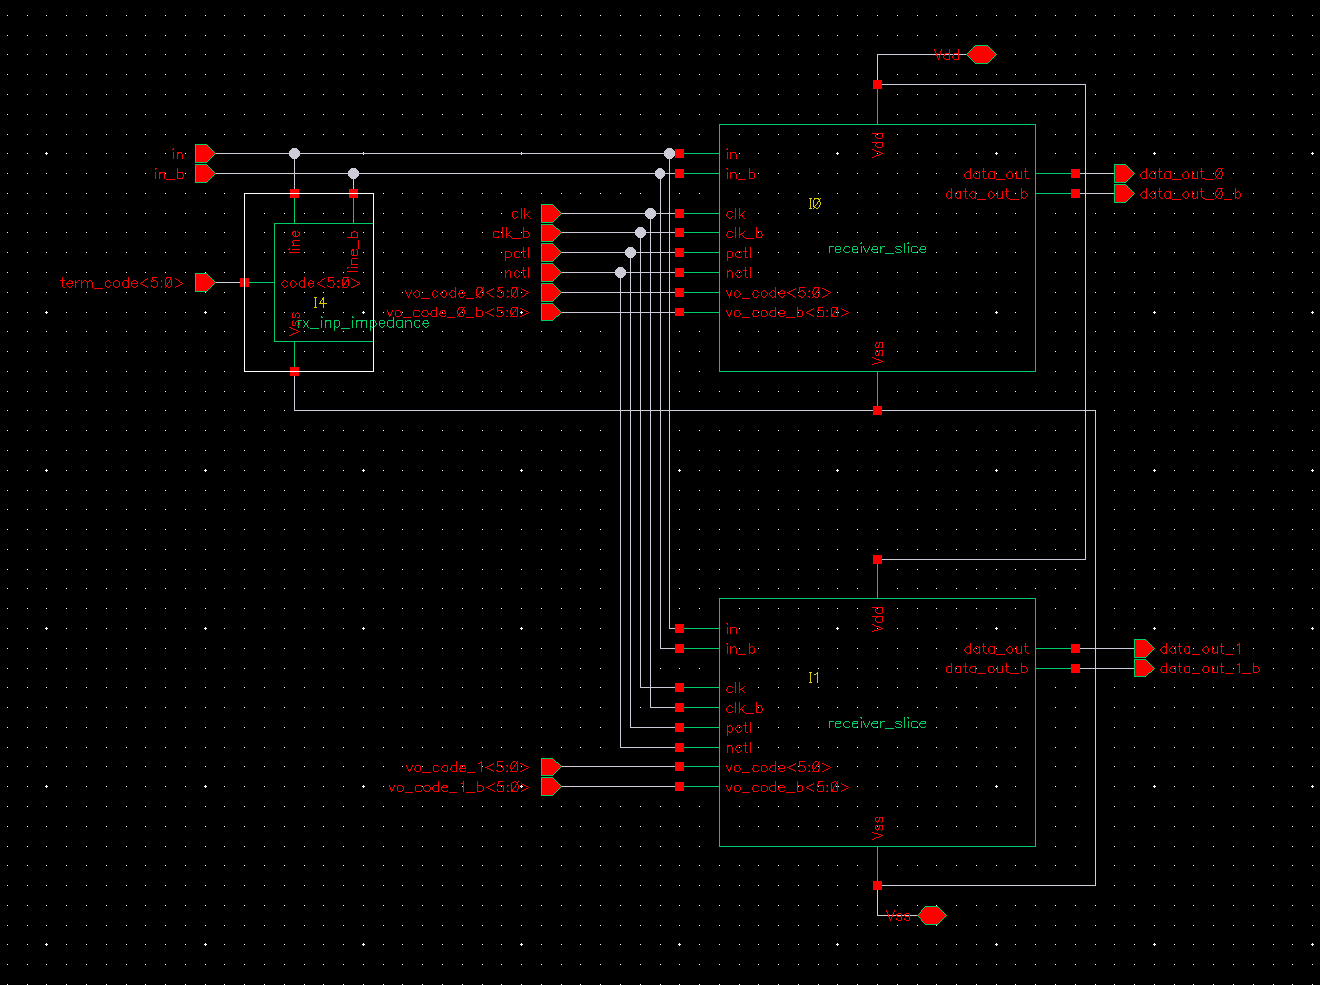
\includegraphics[scale=0.4]{schematics/receiver.png}}
  \caption{Receiver top level circuit}
  \label{fig:top_level}
\end{figure}

\begin{figure}[H]
  \centering
  {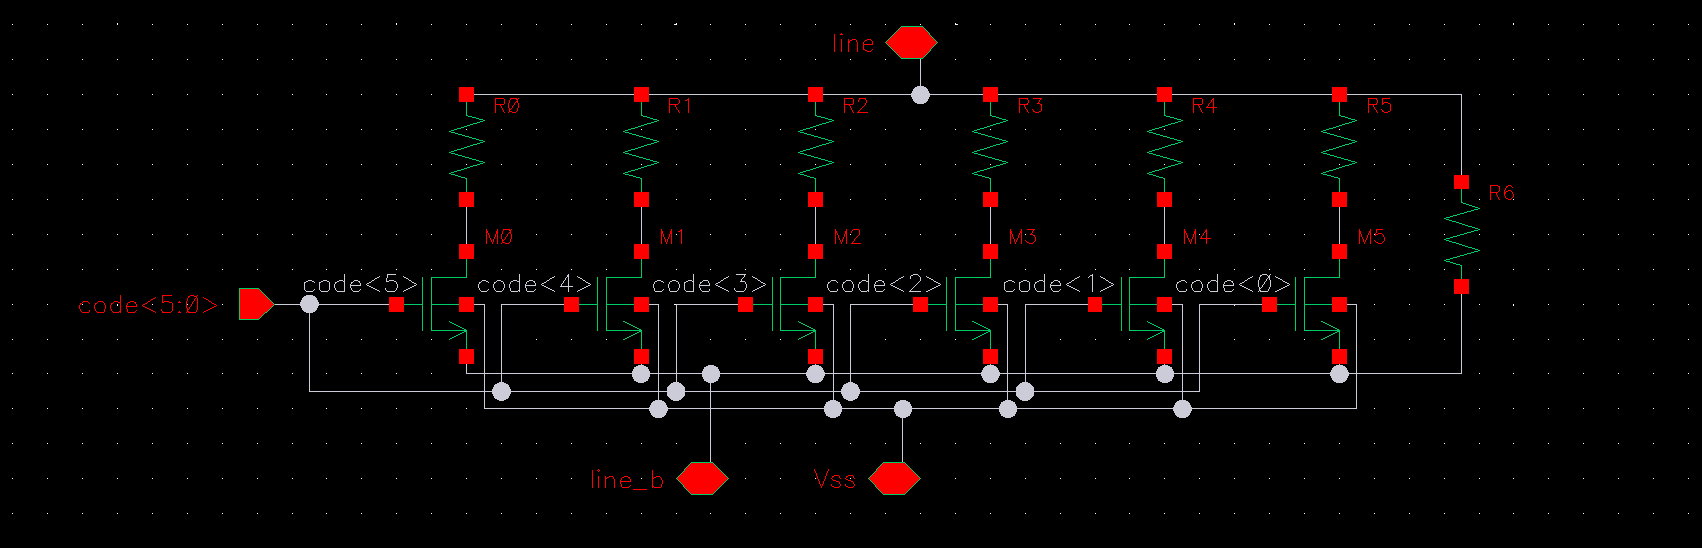
\includegraphics[scale=0.4]{schematics/rx_inp_impedance.png}}
  \caption{Receiver input impedance tuning circuit}
  \label{fig:imp_tuning}
\end{figure}

\begin{figure}[H]
  \centering
  {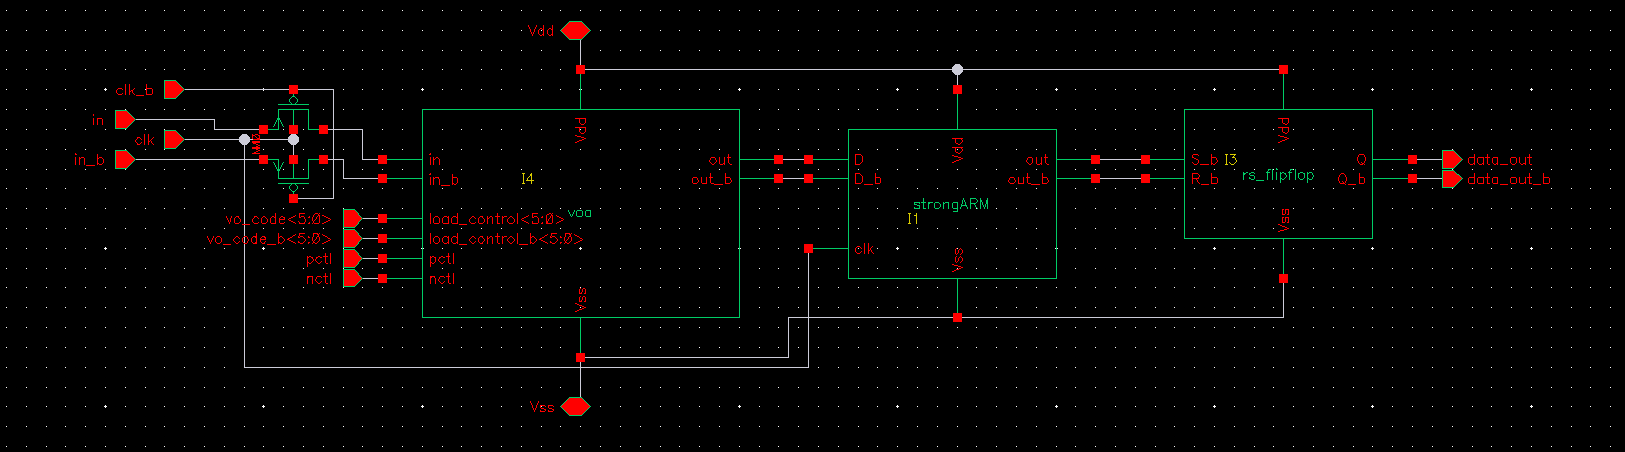
\includegraphics[scale=0.4]{schematics/receiver_slice.png}}
  \caption{Receiver slice circuit}
  \label{fig:receiver_slice}
\end{figure}


\begin{figure}[H]
  \centering
  \subfigure[Variable offset amplifier]
  {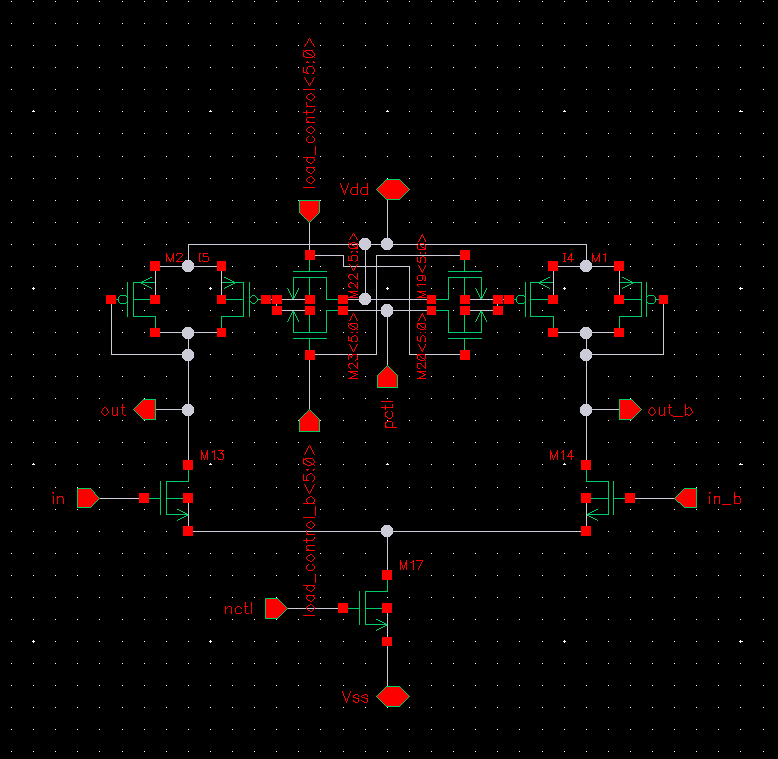
\includegraphics[scale=0.5]{schematics/voa.png}}
  \subfigure[scaled p-channel devices]
  {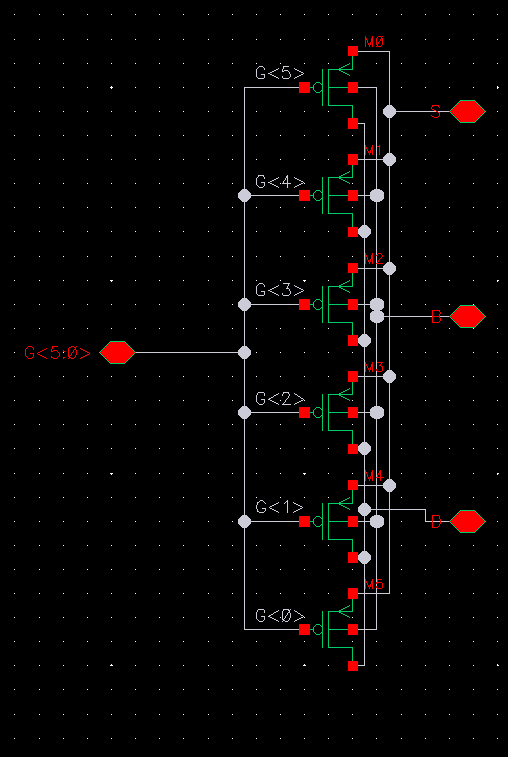
\includegraphics[scale=0.5]{schematics/scaled_pch.png}}
  \caption{Variable offset amplifier (buffer). The devices I4 and I5 are multiple p-channel transistors scaled in size connected like shown in part (b). }
  \label{fig:voa}
\end{figure}

\begin{figure}[H]
  \centering
  {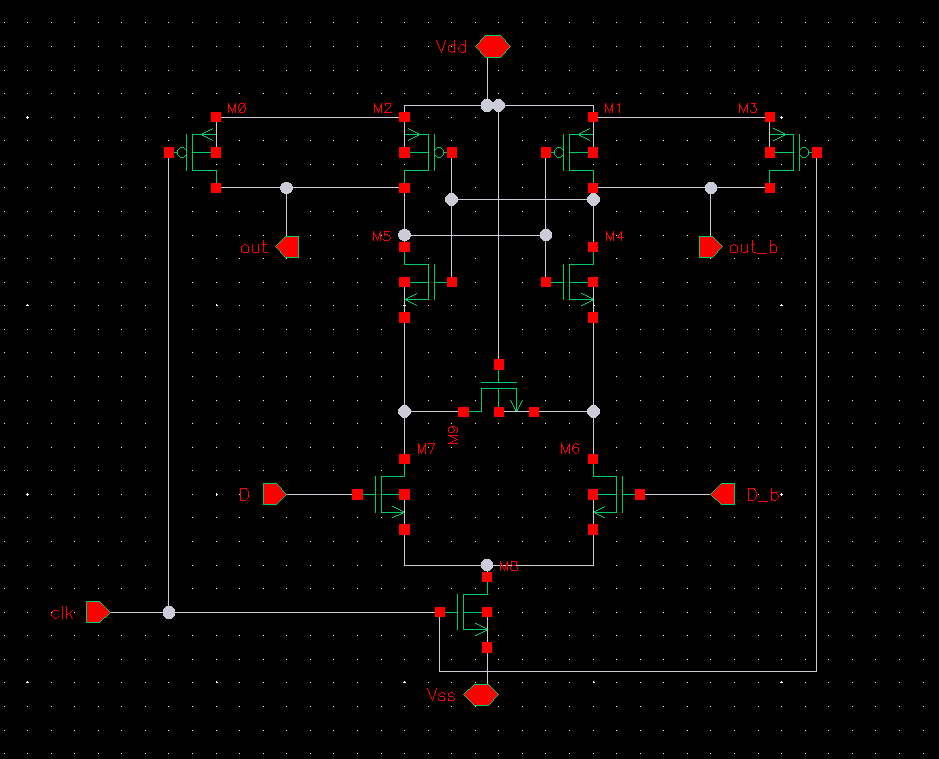
\includegraphics[scale=0.6]{schematics/strongARM.png}}
  \caption{StrongARM latch}
  \label{fig:strongARM}
\end{figure}

\begin{figure}[H]
  \centering
  {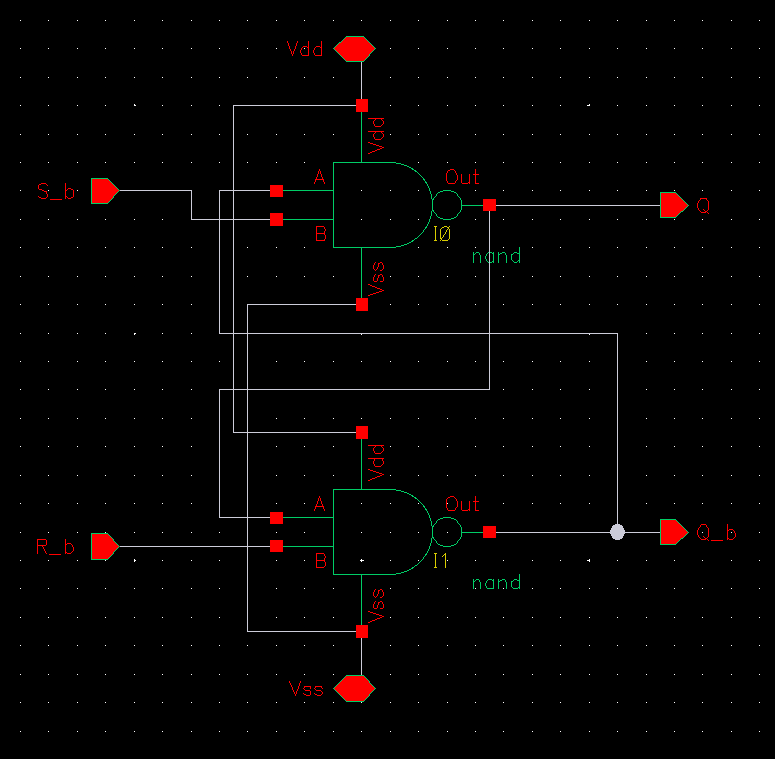
\includegraphics[scale=0.5]{schematics/rs_flipflop.png}}
  \caption{RS-FlipFlop}
  \label{fig:rs_flipflop}
\end{figure}
